% ctexart、ctexrep、ctexbook和ctexbeamer, 对应 LaTeX 的article、report、book和beamer
\documentclass{article}
\usepackage[UTF8]{ctex}
\usepackage[a4paper,left=2cm,right=2cm,top=2.6cm,bottom=2.6cm]{geometry} % 设置页面尺寸
\usepackage{fancyhdr} % 设置页眉页边页脚
\usepackage{multicol} % 多栏排版
\usepackage{xeCJK} % 中文支持
\usepackage{ctex} % 中文支持
\usepackage{footmisc} % 控制脚注格式,包括编号、字体、分隔线等
\usepackage{titletoc} % 定制目录列表样式
\usepackage{fontspec} % XeTeX下的字体选择宏包
\usepackage{setspace} % 行距
\usepackage{graphicx} % 插图
\usepackage{pdfpages} % 引用pdf页面
\usepackage{booktabs} % 三线表
\usepackage{multirow} % 表格多行支持
\usepackage{caption} % figure和table等中的说明文字
\usepackage{tikz} % 绘图
\usepackage{etoolbox} % 给宏包打补丁
\usepackage{hyperref} % 超链接
\usepackage{xcolor} % 颜色支持
\usepackage{array} % 数学表格
\usepackage{amsmath} % 数学公式
\usepackage{amssymb} % 数学字体与符号
\usepackage{amsthm} % 数学定理格式
\usepackage{subfig} % 排版子图
\usepackage{float} % 浮动体格式控制
\usepackage{lmodern} % 一种字体支持
\usepackage{listings} % 插入代码
\usepackage{tcolorbox} % 好看的块环境
\usepackage{pifont} % 字体支持
\usepackage{perpage} %the perpage package
\usepackage{mathdesign} % some math fonts
\usepackage{ulem} %一些文字强调的宏包
\usepackage{fancyvrb} % some fancy verbatim 
\usepackage{enumitem} % 列表项目
\usepackage{txfonts} % 一些字体
\usepackage{makecell}
\usepackage{mathrsfs}
\usepackage{subfig}                 % 子图包,不要与{subfigure}混用,{subfig}较新
\usepackage{overpic}   
\usepackage{auto-pst-pdf}
\usepackage{pst-optexp}
\usepackage{amsmath}
%重置每页脚注序号
\MakePerPage{footnote} %the perpage package command
\renewcommand \thefootnote{\ding{\numexpr171+\value{footnote}}}
\pagestyle{headings} 
% 为tcolorbox导入三个程序包
\tcbuselibrary{skins, breakable, theorems} 

% 设置代码格式 - 关键字加粗, 其余为正常。非彩色
\lstset{
    aboveskip=5mm,
    belowskip=5mm,
    breaklines=true,
    breakatwhitespace=true,
    columns=flexible,
    extendedchars=false,
    showstringspaces=false,
    numbers=none,
    basicstyle={\small\ttfamily},
    captionpos=t,
    frame=tb,
    tabsize=4
}

\lstdefinestyle{cpp} {
  language=C++
}

\lstdefinestyle{c++} {
  language=C++
}

\lstdefinestyle{python} {
  language=python,
  morekeywords={as}
}

% 为目录添加 PDF 链接
\addtocontents{toc}{\protect\hypersetup{hidelinks}}

% 设置「目录」二字格式
\renewcommand{\contentsname}{
  \fontsize{16pt}{\baselineskip}
  \normalfont\heiti{目~~~~录}
  \vspace{-8pt}
}

% 定理、定义、证明
\newtheorem{theorem}{定理}[section]
\newtheorem{definition}{定义}[section]
\newtheorem{lemma}{引理}[section]
\newtheorem{corollary}{推论}[section]
\newtheorem{example}{例}
\newtheorem{proposition}{命题}[section]

\title{光学设计报告}
\author{作者}
\date{\today}

\begin{document}

% 显示标题作者时间
\maketitle
\newpage

% 调整目录行间距
\renewcommand{\baselinestretch}{1.35}
% 添加目录
\tableofcontents
\newpage

% 正文 22 磅的行距
\setlength{\parskip}{0em}
\renewcommand{\baselinestretch}{1.53}


\section{所选题目}
设计透射式望远物镜(为消色差设计,可采用非球面。)
% 
\begin{table}[H]
  \centering
  \begin{tabular}{cc|cc}
  \hline
  参数&数值&参数&数值 \\ \hline
  RMS radius&$<20mrad$&&\\ 
  $2 \omega$&$5^{\circ}$ &$\Gamma$&>2\\ \hline
  \end{tabular}
  \caption{设计参数图}
  \end{table}
\section{对题目内容的分析}
% \section{背景}

% 1609年,意大利天文学家、物理学家伽利略(Galileo di Vincenzo Bonaiuti de' Galilei,1564-02-15~1642-01-08)制作了一个望远镜,采用了凸透镜(正透镜)形式的物镜和凹透镜(负透镜)形式的目镜。这种望远镜成正像,视放大率较小,但视场可以设计成较大。因为成正立的像,在光路中不需要加入倒像(转像)系统。
\subsection{透射式望远镜(开普勒望远镜)}
开普勒望远镜是一种折射式望远镜,由一个凸透镜作为物镜和一个凸透镜作为目镜组成。它的光学原理是利用两个凸透镜的放大效果,将远处的物体形成一个倒立的放大虚像。
开普勒望远镜的优点是\textbf{视野宽,放大倍数更大}。

物镜的像方焦点和目镜的物方焦点重合,位于两透镜之间,形成的像是倒立的实像。出射光瞳在目镜外面,能获得较大的视场。由于成的是实像,它可方便地安置十字丝分划板,以作瞄准、定位和测量之用。
原理图如下所示:
\begin{figure}[H]
    \centering
    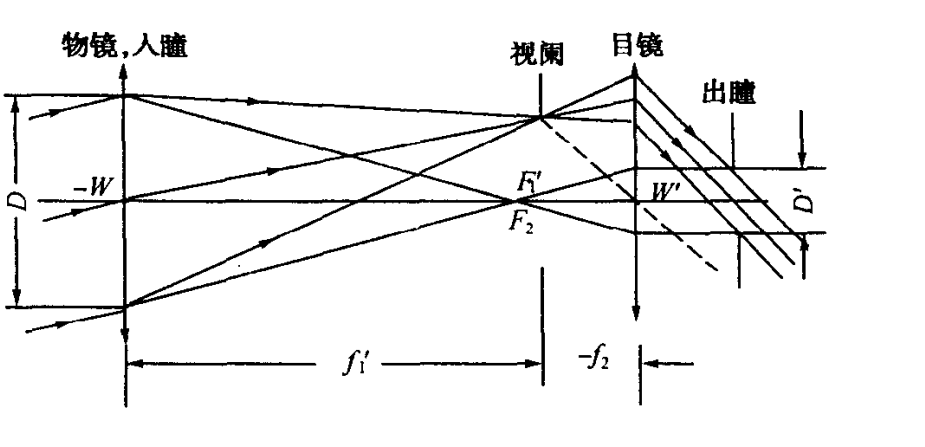
\includegraphics[width=8cm]{img/1.png}
    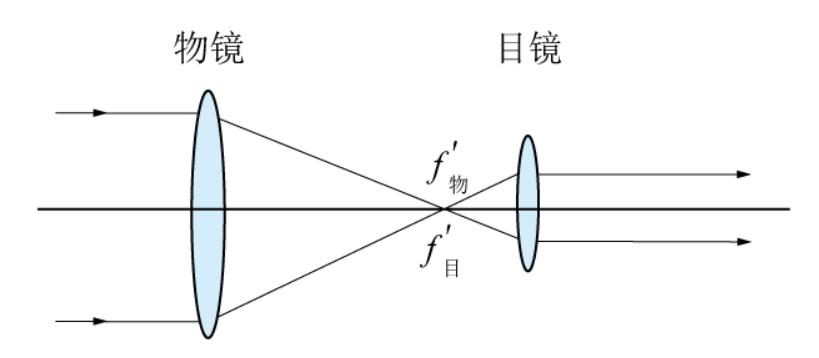
\includegraphics[width=8cm]{img/2.png}
    \caption{原理光路图}
    \end{figure}
        % \begin{figure}[H]
            % \centering
            % \begin{pspicture}[showgrid](4.7,2)
            %     \pnodes(0.7,1){A}(1,1){B}(2.8,1){C}(4,1.5){D}(4,0.5){E}
            %     \psdot[linecolor=gray](A)\psdot[linecolor=gray](B)\psdot[linecolor=gray](C)\psdot[linecolor=gray](D)\psdot[linecolor=gray](E)
            %     \psset{optboxwidth=0.7,labelstyle=\scriptsize}
            %     \addtopsstyle{Fiber}{linecolor=red}
            %     \optbox[position=start,label=0,fiber](A)(B){LD}
            %     \optmzm(B)(C)
            %     \end{pspicture}
            % \end{figure}
% \subsection{望远物镜的主要光学参数}
\subsection{望远物镜的主要光学特性和光学参数}
\begin{description}[leftmargin=1.7cm,style=nextline,nosep]% nosep没有垂直间隔
  \item[相对孔径不大]  在望远系统中,入射的平行光束经过系统以后仍为平行光束
  此物镜的相对孔径( $\displaystyle   \frac{D}{f_{1}^{\prime}} $)和目镜的相对孔径( $\displaystyle   \frac{D^{\prime}}{f_{2}^{\prime}} $)是相等的。目镜的相对孔径主要由出瞳直径
  $ D^{\prime} $和出瞳距离$l'$决定。为了保证出瞳距离,军用望远镜系统的出瞳直径$D'$约为$4mm$,目镜的焦距$ f_{2}' $ 一般大于或等于25mm,这样,目
  镜的相对孔径约为:
  \item[视场角小] 不大于$10^{\circ}$
 \[\frac{D^{\prime}}{f_{2}^{\prime}}= \frac{4}{25}= \frac{1}{6} \]
 \item[望远镜视放大倍率] \[\Gamma= \frac{\tan W^{\prime}}{\tan W}=- \frac{f^{\prime}_{1}}{f^{\prime}_{2}}= \frac{D}{D^{\prime}} \tag{1.1}\] 
\end{description}

\subsection{像差的矫正}

\subsection{需要矫正的像差}
由于望远物镜视为较小,视边缘的成像质量一般允许适当降低。因此望远物镜中都不矫正对应像高$y'$的二次方以上的各种单色像差(像散、场曲、畸变)和垂轴色差,只用校正球差、彗差和轴向色差。
\subsubsection{对不同色光不同的矫正}
望远镜属目视光学仪器,设计目视光学仪器(包括望远镜和显
微镜)一般对F(486.13nm)和C(656.28nm)光计算和校正\textbf{\underline{色差}},
对D(589.3nm)光校正\underline{\textbf{单色像差}}。

\subsubsection{双胶合矫正色差和球差}
望远镜物镜要求校正的像差主要是轴向色差、球差和彗差。由薄透镜
系统的初级像差理论知道,一个薄透镜组除了校正色差所外,还能校正两种单色像差,
刚好符合校正望远物镜像差的需要。

由于双胶合物镜无法矫正像散,场曲,因此它的可用视场一般不超过$10^{\circ}$。

同时查表得到满意成像和相对孔径之间的关系
% 
\begin{table}[H]
  \centering
  \begin{tabular}{|c|cccccc|}
  \hline
  $f_1'$&50&100&150&200&300&100\\ \hline
  $ \frac{D}{f_1'}$ 
  &$ \frac{1}{3}$
  &$ \frac{1}{3.5}$
  &$ \frac{1}{4}$
  &$ \frac{1}{5}$
  &$ \frac{1}{6}$
  &$ \frac{1}{10}$\\ \hline
  \end{tabular}
  \caption{相对孔径表}
  \end{table}
% 这类物镜要达到上述像质要求并无困难,但要求高质量时,要同时校正\textbf{二级光谱和色球差}。可以选用双胶合物镜来减少像差。
% 同时,\textbf{单透镜物镜色差和球差都相当严重}。

% 在玻璃选择得当时,能同时校正色差、球差和彗差,是可能满足像质要求的最简单形式,但胶合面上的高级球差使相对孔径受到限制,且当用普通玻璃时,二级光谱为
% 常量,色球差也无法控制,因而不能获得高的像质。

% 该型式的优点是结构简单,工艺方便,光能
% 损失也小,宜于在焦距不长、相对孔径不大的t场合采用。
同时一般双胶合物镜的最大口径不超过100mm,这是因为当直径过大时,
胶合不牢固,同时当温度改变时,胶台面上容易产生应力,使成像质量变环。

\subsection{像质评价}
\subsubsection{对于色差}
色差是指由于不同波长的光在介质中的折射率不同,导致光的聚焦位置不同,从而影响成像质量的现象。Zemax中分析色差的方法有以下几种:
\begin{enumerate}[label=$\varspadesuit$,nosep]% nosep表示没有垂直间隔
  \item 观察色差曲线的形状和高度
  \item 使用Spot Diagram分析点扩散函数(PSF),观察不同波长的光在像面上的分布情况,以及彩色圆盘的大小和形状。
  \item 观察点列图
\end{enumerate}

% 使用Spot Diagram分析点扩散函数(PSF),观察不同波长的光在像面上的分布情况,以及彩色圆盘的大小和形状。
使用Wavefront Map分析波前图,观察不同波长的光在像面上的相位差情况,以及色差引起的波前畸变。
使用MTF Plot分析调制传递函数(MTF),观察不同波长的光对系统分辨率的影响,以及色差对MTF曲线的降低。
使用Chromatic Focal Shift分析色散焦移,观察不同波长的光在系统中的最佳聚焦位置,以及色散焦移量和方向。
\section{Zemax设计的过程及设计结果}
\subsection{根据设计要求选择整体结构}
因为是消色差设计(单透镜的色差和单色像差很大),同时根据望远镜的常见结构,我们显然选择两个双胶合透镜,一个作为物镜,一个作为目镜。接下来我们需要在老师给出的玻璃库中选取合适的玻璃,一个作为目镜,一个作为物镜。
结构如图1原理光路图所示。
\begin{quote}
{\qquad\parindent2\ccwd\kaishu\zihao{5}
选定玻璃后,只能调空气厚度。实际光路要求轴长不超1m,空气厚度不低于25mm。
}
\end{quote}

\subsection{玻璃的计算和选取}
给出可用的玻璃如下:
% 
\begin{table}[H]
  \centering
  \begin{tabular}{|c|cccc|}
  \hline
  序号&型号&品名&规格&相对孔径\\ \hline
  1&GCL-010604&
  双胶合消色差透镜&
  $\Phi 25.4 \hspace{0.2cm}  f100.0$& 0.254\\
  2&GCL-010606&
  双胶合消色差透镜&
  $\Phi 25.4 \hspace{0.2cm}  f 200.0$& 0.127\\
  % Φ25.4,f200.0\\ \hline
  3&GCL-010615&
  双胶合消色差透镜&
  % Φ50.8.f100.0\\ \hline
  $\Phi 50.8 \hspace{0.2cm}  f 100$& 0.508\\

  4&GCL-010617&
  双胶合消色差透镜&
  % Φ50.8.f200.0\\ \hline
  $\Phi 50.8 \hspace{0.2cm}  f 200$& 0.254\\

  5&GCL-010631&
  双胶合消色差透镜&
  % Φ30.0,f75.0\\ \hline
  $\Phi 30 \hspace{0.2cm}  f 75$& 0.4\\

  6&GCL-010632&
  双胶合消色差透镜&
  % Φ30.0.f90.0\\ \hline
  $\Phi 30 \hspace{0.2cm}  f 90$& 0.33\\

  7&GCL-010640&
  双胶合消色差透镜&
  % Φ40.0,f120.0\\ \hline
  $\Phi 40 \hspace{0.2cm}  f 120$& 0.33\\

  8&GCL-010641&
  双胶合消色差透镜&
  % Φ40.0,f250.0\\ \hline
  $\Phi 40 \hspace{0.2cm}  f 250$& 0.16\\

  9&GCL-010642&
  双胶合消色差透镜&
  % Φ40.0,f300.0\\ \hline
  $\Phi 40 \hspace{0.2cm}  f 300$& 0.133\\

  10&GCL-010650&
  双胶合消色差透镜&
  % Φ25.4.f30.0\\ \hline
  $\Phi 25.4 \hspace{0.2cm}  f 30$& 0.847\\

  11&GCL-010654&
  双胶合消色差透镜&
  % Φ25.4.f75.0\\ \hline
  $\Phi 25.4 \hspace{0.2cm}  f 75$&0.472\\

  12&GCL-010656&
  双胶合消色差透镜&
  % Φ25.4,f175.0\\ \hline
  $\Phi 25.4 \hspace{0.2cm}  f 175$&0.145\\ \hline
  
  % 13&GCL-010713&双胶合消色差负透&
  
  % Φ25.4,f50.0 \\ \hline
 
  % 14&GCL-010714&双胶合消色差负透 镜&
  
  % Φ25.4.f-75.0 \\ \hline

  \end{tabular}
  \caption{可用玻璃列表}
  \end{table}
  首先选择物镜,其相对孔径要满足表2.故首先排除掉3,5,6,10,11.
        % \begin{figure}[H]
        %     \centering
        %     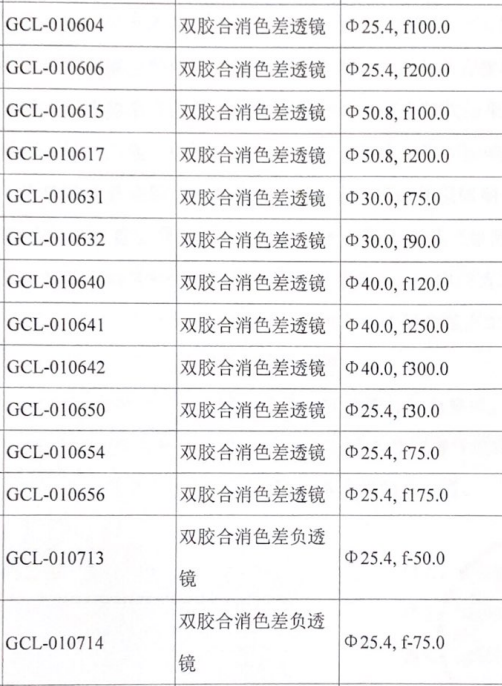
\includegraphics[width=8cm]{img/4.png}
        %     \caption[]{可用玻璃列表}
        %     \end{figure}

首先要满足物镜焦距$f_1'$满足
\[f_1'>2f_2'\]
并且双胶合物镜的选择要满足相对孔径,在剩下的里面选择相对孔径较小的GCL-010606作为物镜。再选择GCL-010631作为目镜。他们的关键参数如下
\begin{table}[H]
  \centering
  \begin{tabular}{cccccccc}
  \hline
  类型&型号&品名&规格&$\Phi$&$R1$&$R 2$&$R 3$ \\ \hline
  物镜&GCL-010606
  &双胶合消色差透镜
  &$\Phi25.4,f200.0$ &
  25.4
  &
  119.758
  &
  -90.616
  &-277.773\\ \hline \hline
  双凸边缘厚&
弯月边缘厚&双凸中心厚&
弯月中心厚&
双凸材料&
弯月材料&$T_c$&$T_e$ \\ \hline
2.03&
3.104&
3.6&
2.5&
H-K9&
H-ZF2&6.1&5.1\\ \hline\hline
类型&型号&品名&规格&$\Phi$&$R1$&$R 2$&$R 3$ \\ \hline
  目镜&GCL-010631
  &双胶合消色差透镜
 & $\Phi30.0,f75.0$&30&
 
 44.118&-34.554&-106.839
 \\ \hline \hline
 双凸边缘厚&
弯月边缘厚&双凸中心厚&
弯月中心厚&
双凸材料&
弯月材料&$T_c$&$T_e$ \\ \hline 
1.846&
4.367&
7.9&
2&
H-K9&
H-ZF2&
9.9&
6.2\\ \hline
  \end{tabular}
  \caption{透镜选择及其参数(偶数行是数值,奇数行是内容)}
  \end{table}
          \begin{figure}[H]
              \centering
              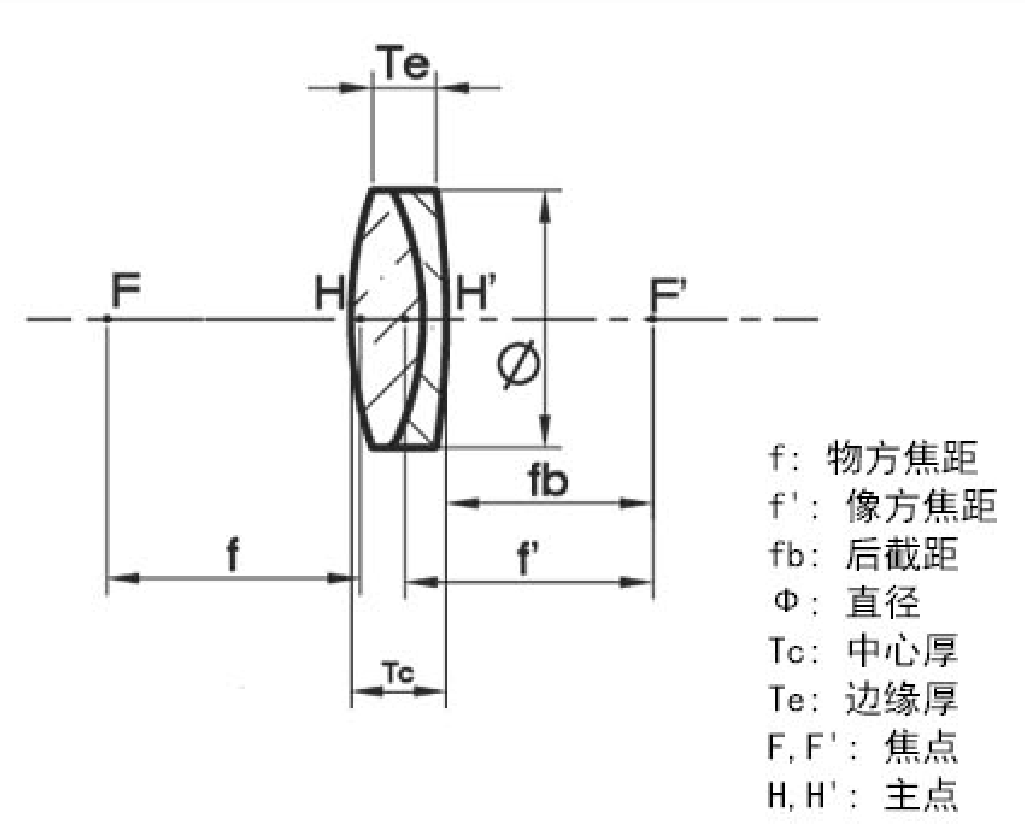
\includegraphics[width=8cm]{img/3.png}
              \caption[]{透镜参数示意图}
              \end{figure}

同时经过计算初始像差,其较小,满足要求。
\subsection{数据分析}
% 选择的物镜和目镜分别为:(默认单位(mm))

计算一些参数如下
\begin{description}[leftmargin=1.7cm,style=nextline,nosep]% nosep没有垂直间隔
  \item[视觉放大倍率] \[\Gamma=- \frac{f_1^{\prime}}{f_2^{\prime}}=-\frac{200}{75}=-2.667  \tag{1.2}\] 
  \item[镜筒长度 $\thickapprox=f+f'=275mm$]
  \item[入瞳直径$D$]
  \[D=25.4 mm \tag{1.3}\]
  \item[出瞳直径$D'$] \[D'=30 mm\tag{1.4}\]
  % \item[像方视场角$\omega'$]
  % \item[目距]
  % \item[]   
  % \item[]   
\end{description}
\subsection{zemax操作和基本设置}
按照选取的初始结构,将镜头数据输入zemax中的镜头数据中。并且设置视场角,以及光线追迹的参数,波长。(这里我们使用zemax2021进行演示,因为其更加人性化)
\subsection{镜头参数的设置}
\begin{quote}
{\qquad\parindent2\ccwd\kaishu\zihao{5}
在zemax中,如果材料不为空,那么表示空气层。厚度表示该面到下一个面的中心厚度。
}
\end{quote}
对于双胶合透镜如(图2透镜参数示意图)以及(表 4: 透镜选择及其参数)所示,其需要填写三个面的半径以及两个面的厚度,一个
双凸边缘厚,一个弯月中心厚。同时根据初始结构,我们需要设置两个透镜的距离,即物镜的后表面到目镜的前表面的距离,根据开普勒望远镜的特点,设置为$275mm$,并将其设置为变量进行优化。
% 
\begin{table}[H]
  \centering
  \begin{tabular}{ccccc}
  \hline
  表面类型&表面标注&曲率半径&厚度&材料\\ \hline
  标准面	&	物面&$\infty$&$\infty$&\\ 
  标准面	&物镜前表面	&119.758	&3.6& H-K9\\ 
  标准面	&胶合面	&-90.616	&2.5&	H-ZF2\\ 
  标准面	&物镜后表面	&-277.773	&275& (空气)\\ 
  标准面	&目镜前表面	&44.118&7.9&H-K9\\ 
  标准面	&胶合面	&-34.554&2&H-ZF2\\ 
  标准面	&目镜后表面	&-106.839&$\infty$&(空气)\\ 
  标准面	&	像面&$\infty$&$\infty$&\\ \hline

  

\end{tabular}
  \caption{镜头参数表}
  \end{table}
          \begin{figure}[H]
              \centering
              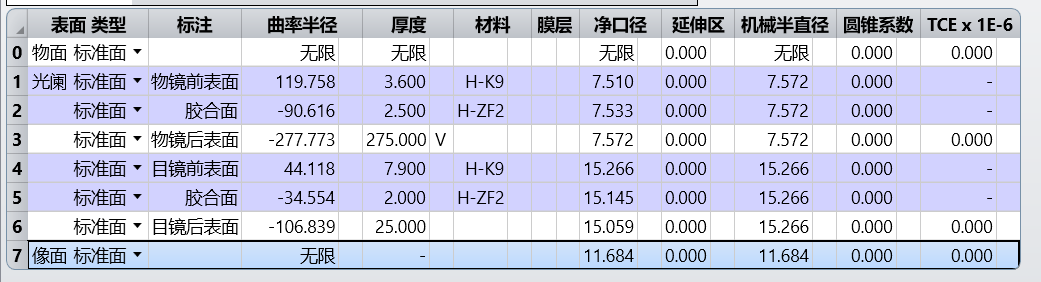
\includegraphics[width=18cm]{img/5.png}
  \caption{镜头参数填写示意图}
              \end{figure}
  \begin{quote}
  \end{quote}
\subsubsection{系统孔径,光线追迹参数的设置以及其他杂项}
入瞳直径为物镜直径,设置入瞳直径为$30mm$,并勾选无焦像空间
\footnote{在Zemax中,"无焦像空间模式"是一种模拟光线在光学系统中传播的方式。该模式考虑了光线在非理想光学元件(例如透镜)中的传播过程,以及由此引起的畸变和像差。

在无焦像空间模式下,Zemax会通过模拟光线的传播路径来计算系统中的像差。这些像差包括球差、彗差、色差、像场曲率等。通过分析这些像差,可以优化光学系统设计,以改善成像质量。}。
\begin{figure}[H]
  \centering
  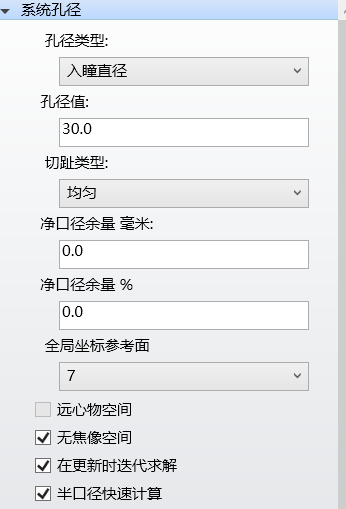
\includegraphics[width=4cm]{img/6.png}
  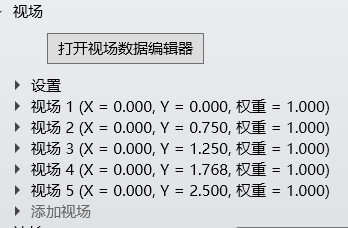
\includegraphics[width=6cm]{img/7.png}
  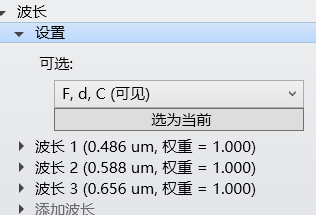
\includegraphics[width=6cm]{img/8.png}

\caption{系统孔径设置(左),追迹光线视场设置(中),追迹光线波长设置(右)}
  \end{figure}
  一般设置视场角都是按照带区设置:0、0.3、0.5、0.707、1(常用这5个带)比如你的系统的全视场是20度,那么半视场是10度,输入zemax的5个带区分别为:0度、3度、5度、7、07度、10度也没有必要非要输入5个带区,可多可少但是0带、0.707带和最边缘的1带最好有,这3个带很有实际价值。
  这里我们的全视场$5^{\circ}$,所以我们对半视场分别乘为0、0.3、0.5、0.707、1,得到追迹光线视场设置。

  波长就使用常见的$F,d,c$光。
\subsection{基础分析}
完成上述操作后,我们查看系统光路图以及查看系统报告和一些其他曲线,检验系统是否满足要求。
\begin{figure}[H]
  \centering
  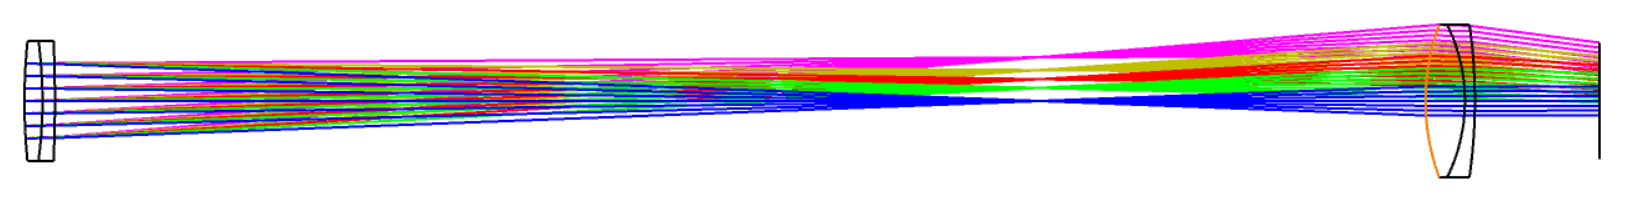
\includegraphics[width=18cm]{img/9.png}
\caption{2D系统光路示意图}
  \end{figure}
  % 
  \begin{table}[H]
    \centering
    \begin{tabular}{|cc|c c|cc|}
    \hline
    名称&数据&名称&数据& 名称&数据\\ \hline
    总长&316&近轴放大率&0&入瞳位置&0\\ 
    出瞳直径& 11.04874&出瞳位置&72.38755&最大径向视场 &2.5\\
    主波长&0.5875618 μm&角放大率&-2.715241&透镜单位&毫米\\ 
    \hline
    \end{tabular}
    \caption{系统数据}
    \end{table}

  同时注意到这里由于我们使用的物方光线是平行光束,所以近轴放大率\footnote{近轴像平面上的近轴主光线高与物高的比值}为0。
          \begin{figure}[H]
              \centering
              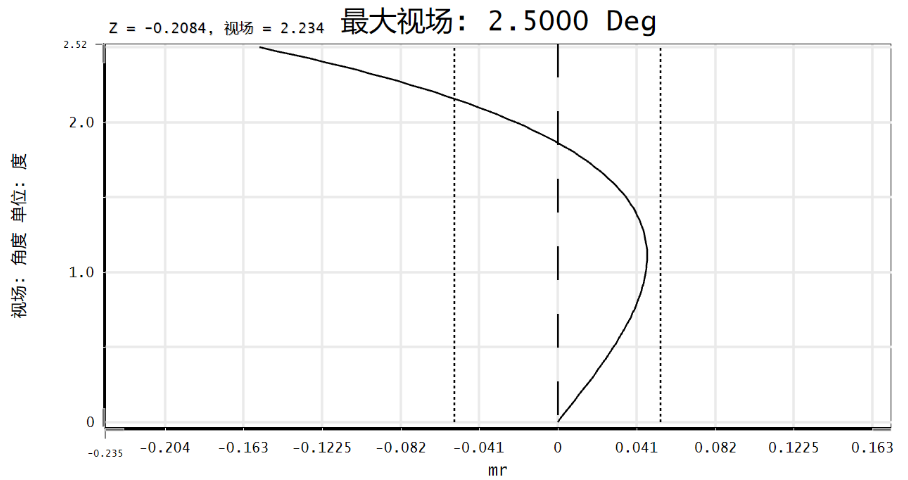
\includegraphics[width=12cm]{img/10.png}
\caption{在F光C光下的色差曲线}
              \end{figure}
              \begin{figure}[H]
                \centering
                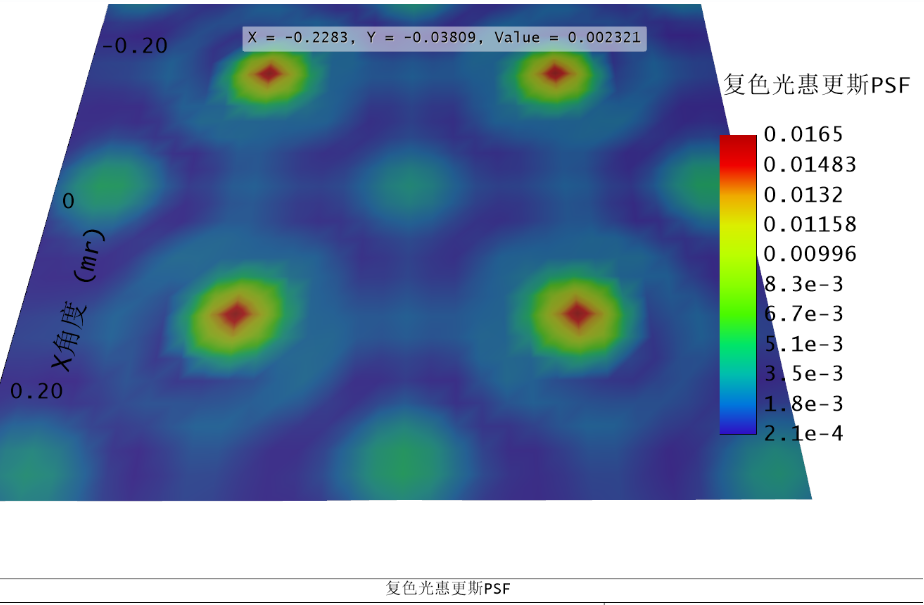
\includegraphics[width=12cm]{img/11.png}
  \caption{复色光惠更斯PSF}
                \end{figure}

                \begin{figure}[H]
                  \centering
                  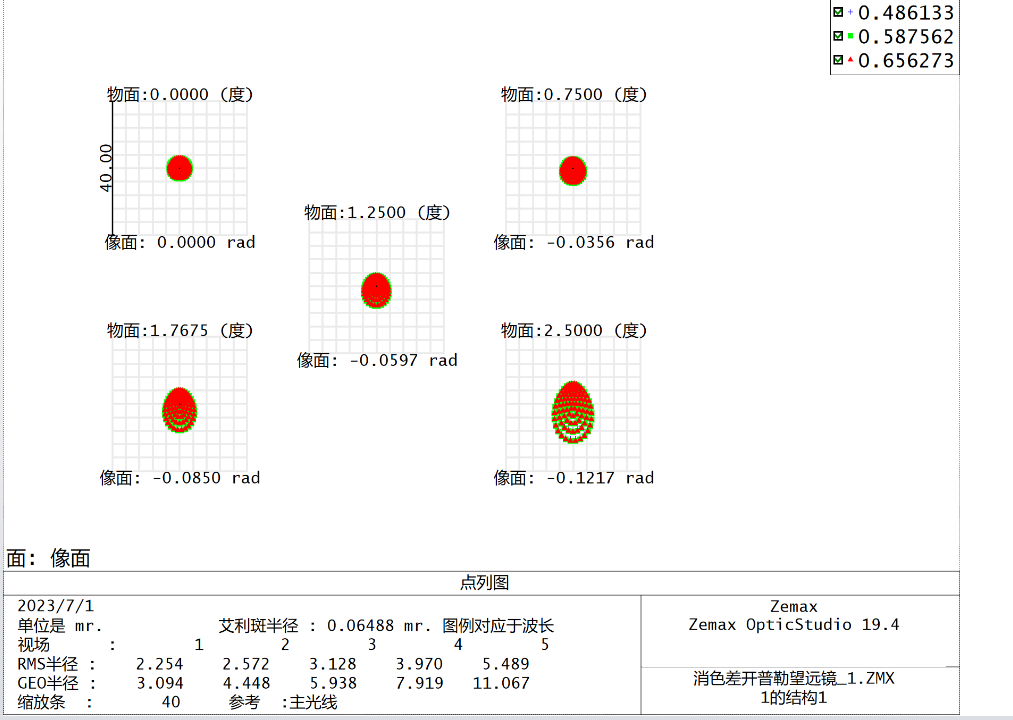
\includegraphics[width=18cm]{img/13.png}
    \caption{标准点列图以及RMS半径}
  \end{figure}

    \begin{figure}[H]
      \centering
      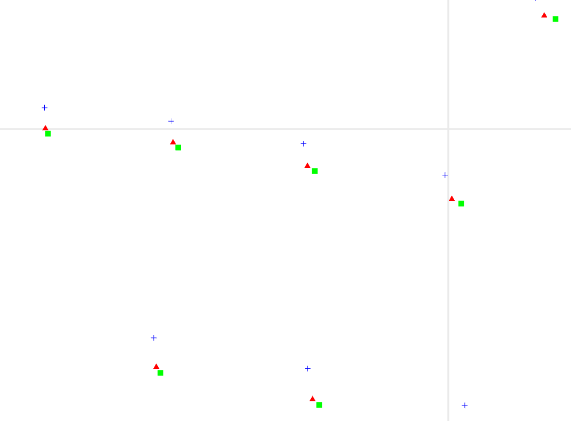
\includegraphics[width=8cm]{img/14.png}
\caption{点列图放大(观察色差)}
                  \end{figure}

                  \begin{figure}[H]
                    \centering
                    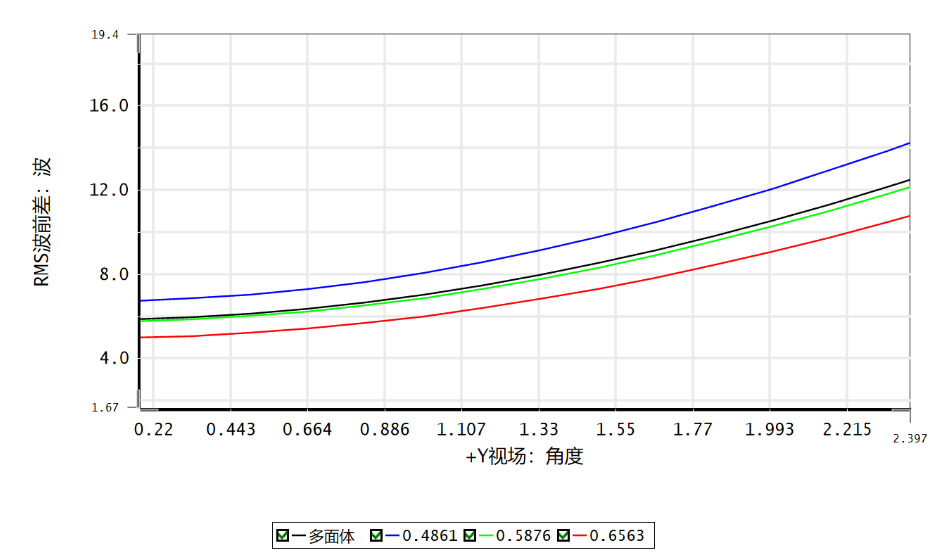
\includegraphics[width=15cm]{img/15.png}
              \caption{RMS-视场}
                                \end{figure}
                                \begin{figure}[H]
                                  \centering
                                  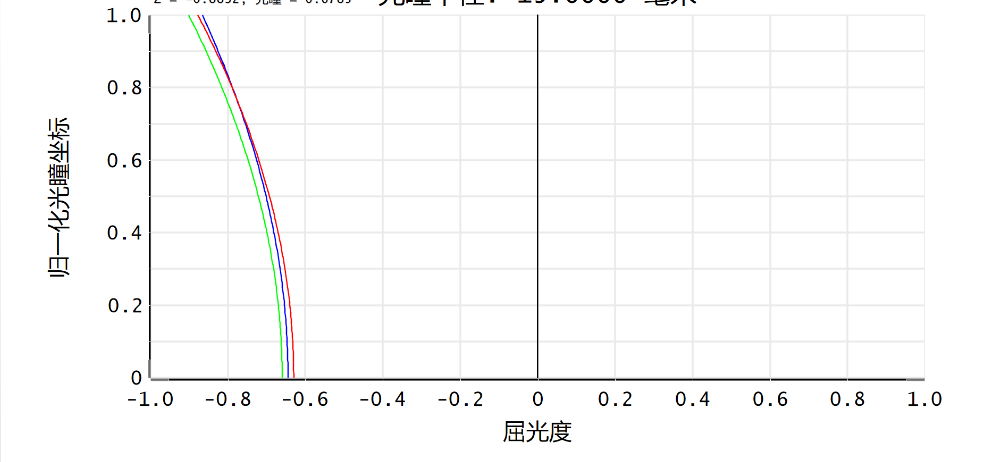
\includegraphics[width=15cm]{img/16.png}
                            \caption{未校正的轴向像差}
                                              \end{figure}        
显然根据以上各图我们可以看到色差得到了很好的消除,我们完成了消除色差的设计。
同时$RMS_{NAX} < 20mrad$,也满足设计要求。
但是\textbf{轴向像差还是很大},所以我们需要对其进行校正。我们将两透镜之间的空气厚度设置为变量,并使用zemax进行自动优化。
\subsection{系统优化}
前文中变量已设置完成。在设置变量完成后需要进行评价函数的设置,
% 点击编辑器-评价函数,点击设计-自动序列评价函数,勾选空气厚度最小设置为25。
一旦设置好变量,现在就可以构造默认的评价函数(Merit Function)。
评价函数是在一个完全独立于镜头数据编辑器的编辑器中构造的,称为评价函数编辑器(Merit Function Editor)。
通过点击:优化 (Optimize)> 评价函数编辑器(Merit Function Editor),打开评价函数编辑器。

评价函数(Merit Function)
是光学系统与指定目标的接近程度的数值表示。

在评价函数编辑器中,OpticStudio使用操作数列表,这些操作数分别代表系统的不同约束或目标。
当评价函数构建完成后,OpticStudio中的优化算法会尝试使评价函数的值尽可能小。

虽然您可以自己构建评价函数,但是让OpticStudio为您构建评价函数更加容易。
默认的评价函数可以通过从评价函数编辑器的菜单栏选择优化向导与操作数(Wizards and Operands)>
优化向导( Optimization Wizard )来构建。


选择此选项后,将出现优化向导(Optimization Wizard)对话框,
可以从中选择各种选项来定义默认的评价函数。我们选择针对相对于质心的RMS半径进行优化,
所有这些选项都已经内置到OpticStudio的优化向导中。

为了防止单透镜变得太厚或太薄,对该透镜的厚度设置边界约束是很重要的。
在优化向导(Optimization Wizard)中,可以在厚度边界(Boundary Values)部分设置玻璃和空气厚度的边界约束。通过“空气(Glass)”选项,可以将最小、
最大和边缘厚度值手动输入到适当的条目中。此处我们设置其在\textbf{260-280}之间变化。
        \begin{figure}[H]
            \centering
            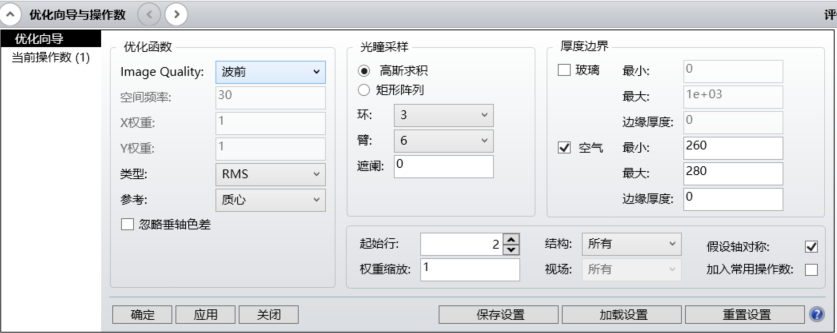
\includegraphics[width=10cm]{img/17.png}
            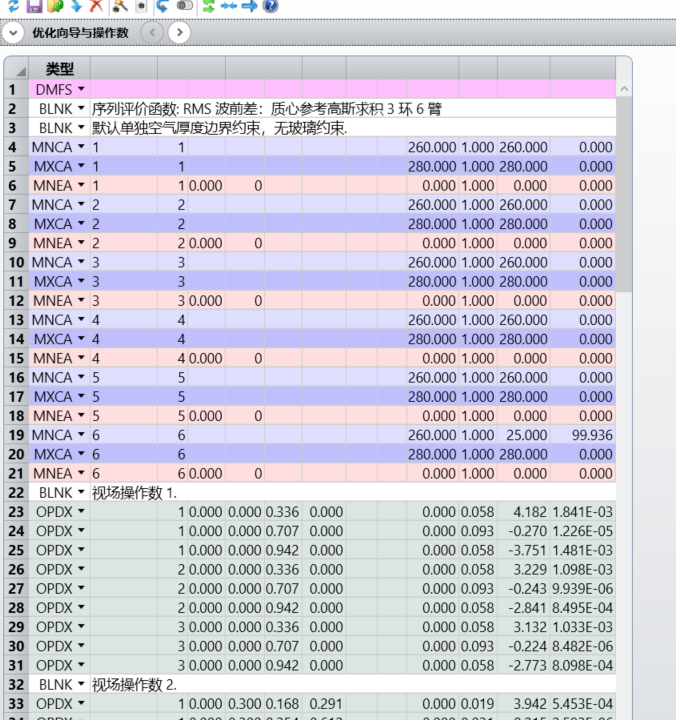
\includegraphics[width=5cm]{img/18.png}
            \caption{评价函数助手(做)及自动生成的评价函数}

            \end{figure}
            \begin{figure}[H]
              \centering
              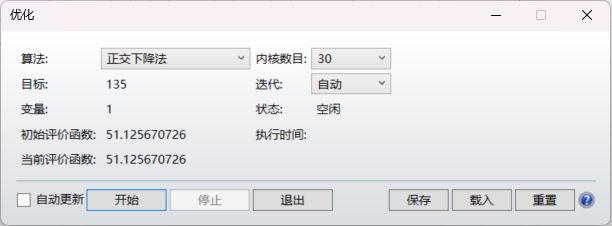
\includegraphics[width=13cm]{img/22.png}
              % 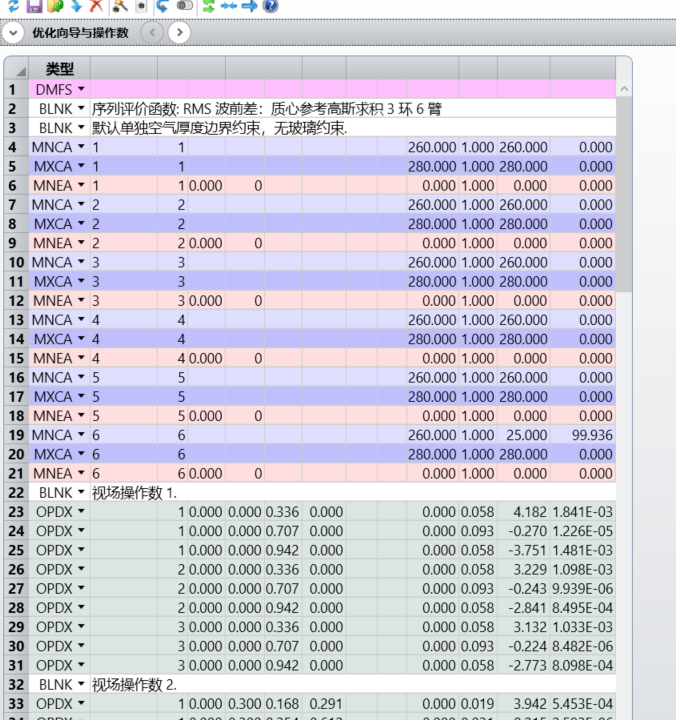
\includegraphics[width=5cm]{img/18.png}
              \caption{优化过程示意图}
  
              \end{figure}
自动优化之后,系统参数如下
% 
\begin{table}[H]
  \centering
  \begin{tabular}{cccccc}
  \hline
  空气厚度&269.101mm&$RMS_{MAX}$& 1.41378057E+00 mr&角放大率& -2.637129\\ \hline
  \end{tabular}
  \caption{优化后系统参数表}
  \end{table}
以下为优化后的效果图
\begin{figure}[H]
  \centering
  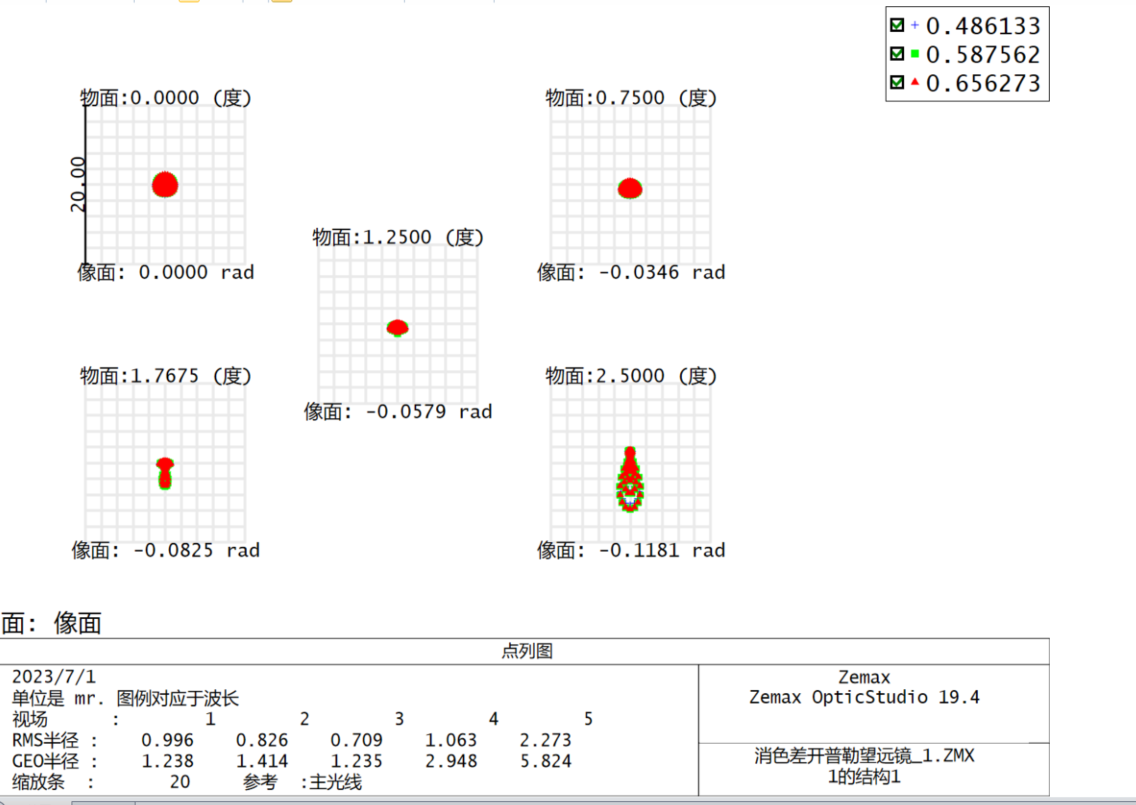
\includegraphics[width=16cm]{img/19.png}
  % 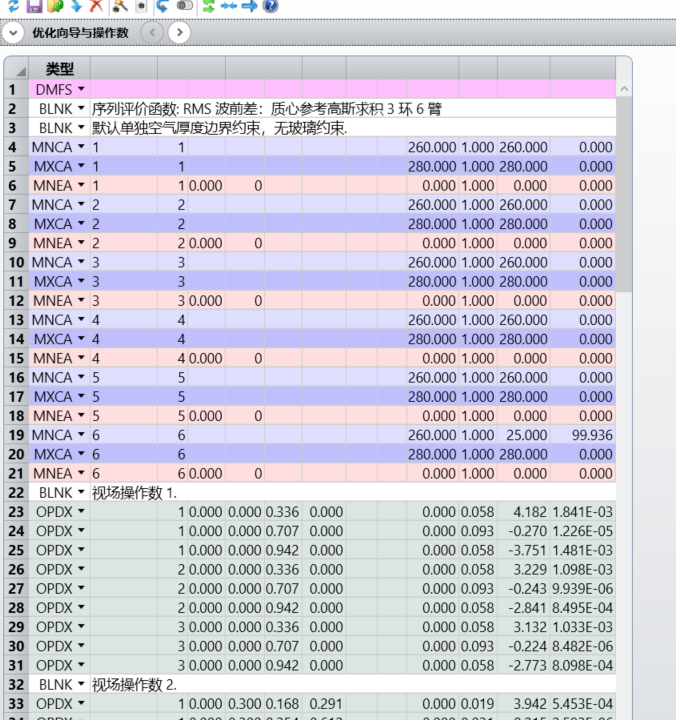
\includegraphics[width=5cm]{img/18.png}
  \caption{优化后标准点列图}

  \end{figure}

  \begin{figure}[H]
    \centering
    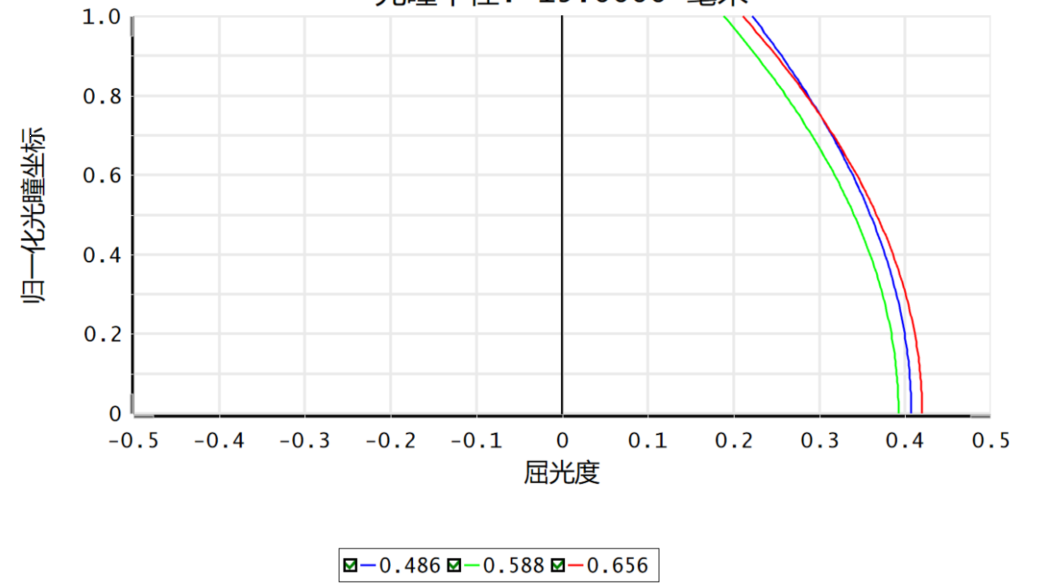
\includegraphics[width=16cm]{img/20.png}
    % 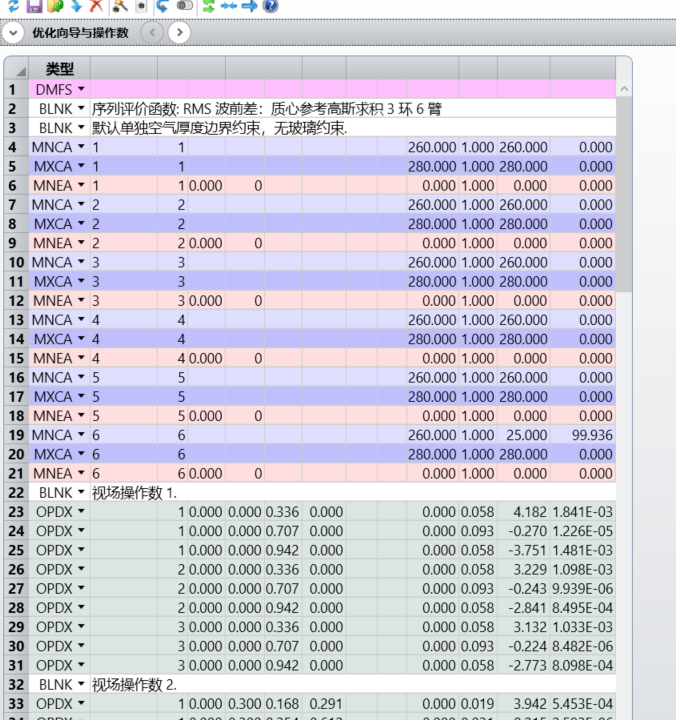
\includegraphics[width=5cm]{img/18.png}
    \caption{优化后轴向色差示意图}
  \end{figure}

  \begin{figure}[H]
    \centering
    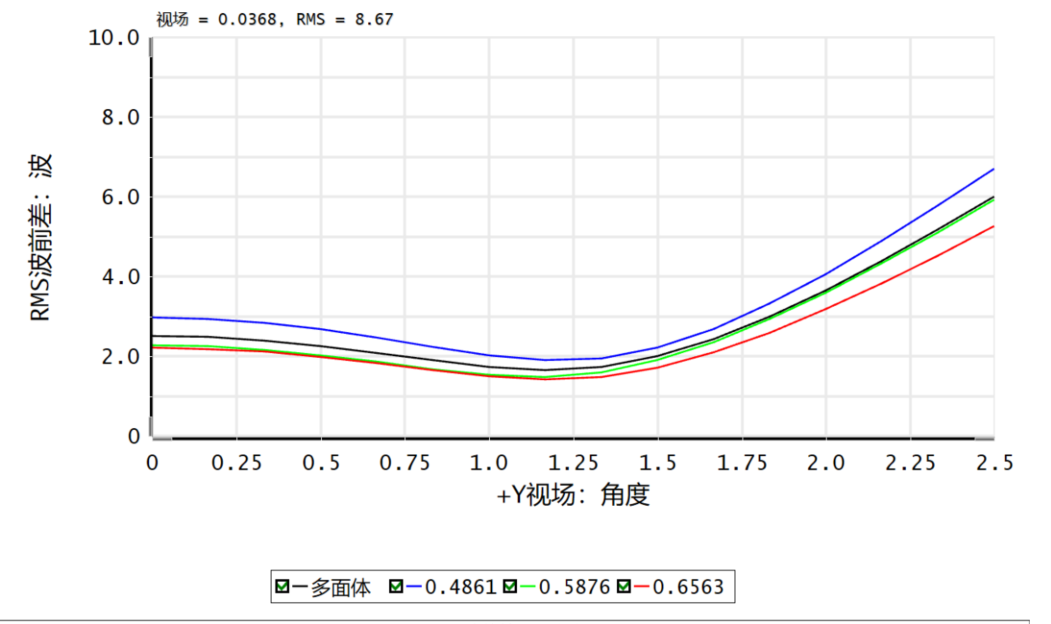
\includegraphics[width=16cm]{img/21.png}
    % 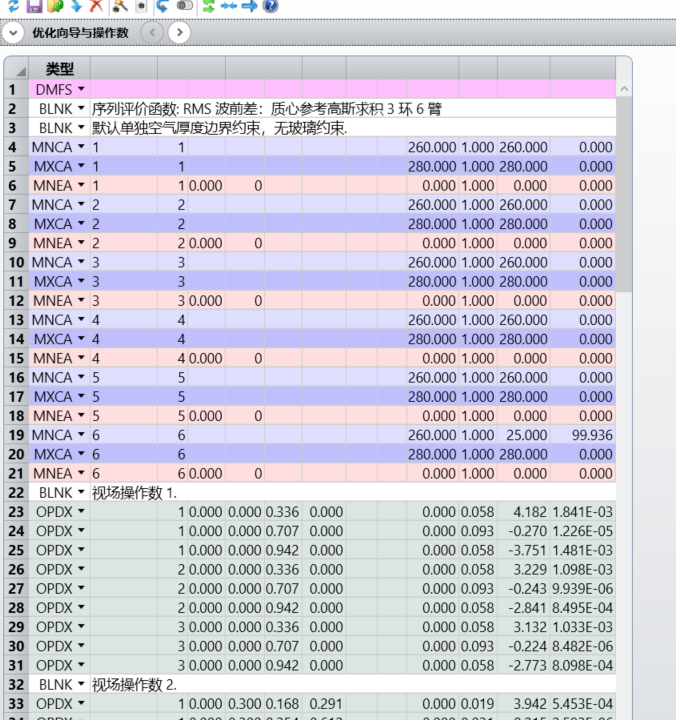
\includegraphics[width=5cm]{img/18.png}
    \caption{优化后RMS示意图}
  \end{figure}
  至此优化完毕,题目要求的设计要求全都满足,并且色差和轴向色差均比较小。

\section{光路的搭建(要严格按照设计结果进行搭建,如果有改动要说明)}
\subsection{实际搭建}
我们小组在按照Zemax仿真设计的结果选择玻璃,搭建,调整,十分顺利,实际效果明显,无差错。
\begin{figure}[H]
  \centering
  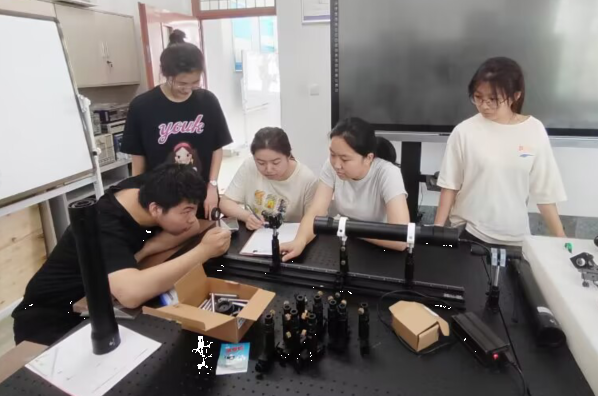
\includegraphics[width=16cm]{img/24.png}
  % 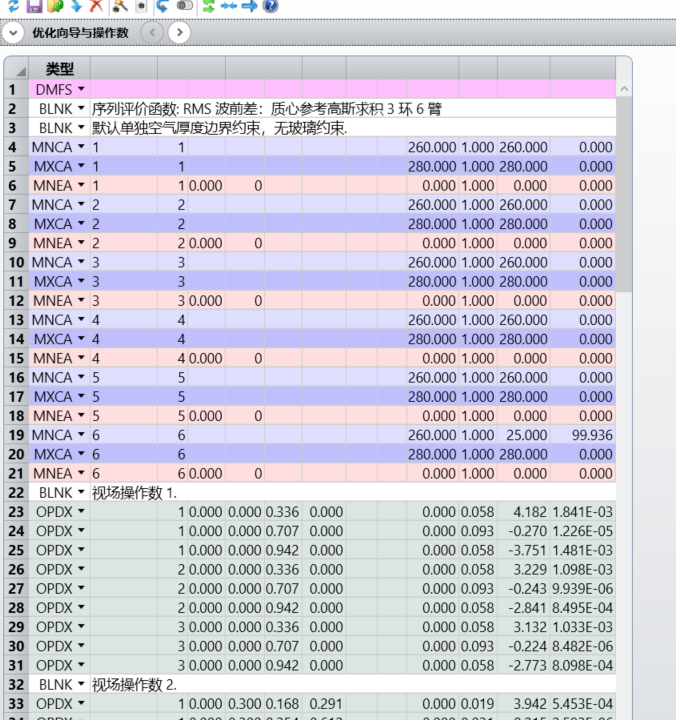
\includegraphics[width=5cm]{img/18.png}
  \caption{合照以及光路示意图(正在观测)}
\end{figure}
\section{搭建的光路是否实现了设计的目标(需要把搭建的光路以及最后所成的像,用照片或者图片的方式放到报告当中)}
\begin{figure}[H]
  \centering
  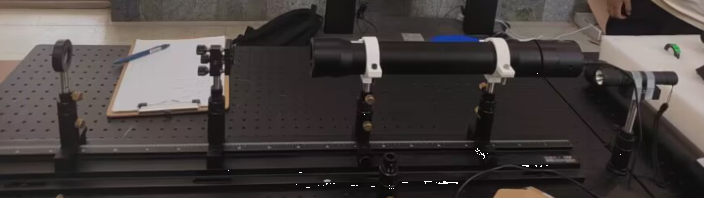
\includegraphics[width=16cm]{img/23.png}
  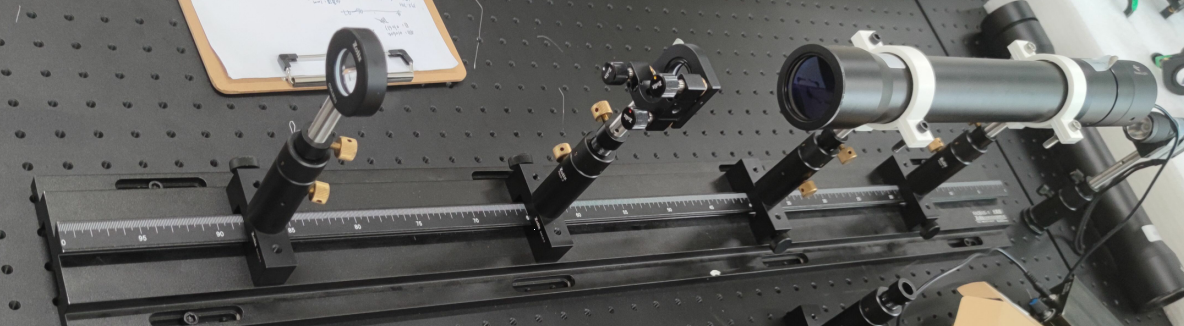
\includegraphics[width=16cm]{img/25.png}

  % 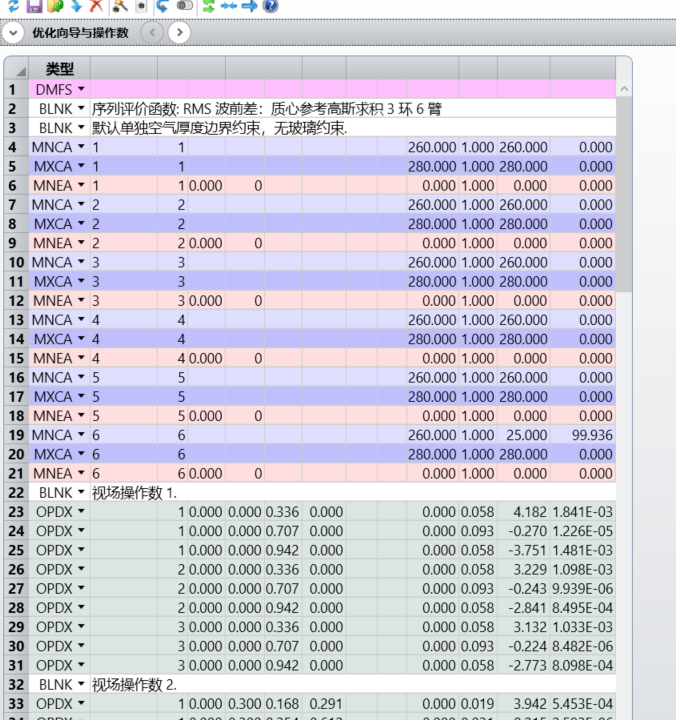
\includegraphics[width=5cm]{img/18.png}
  \caption{搭建的光路示意图}
\end{figure}
\begin{figure}[H]
  \centering
  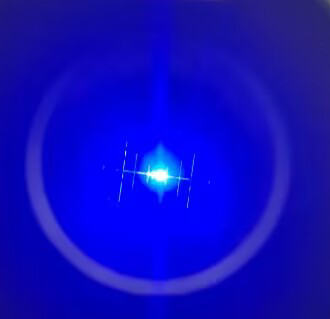
\includegraphics[width=6cm]{img/26.png}
  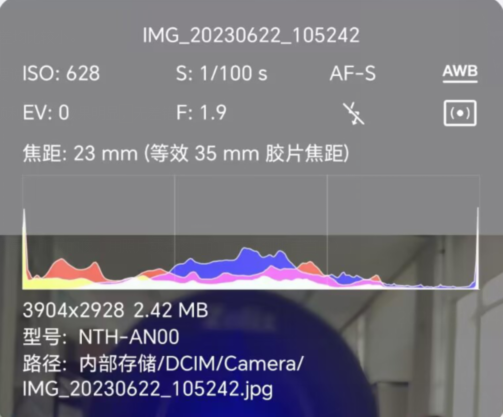
\includegraphics[width=7cm]{img/27.png}

  % 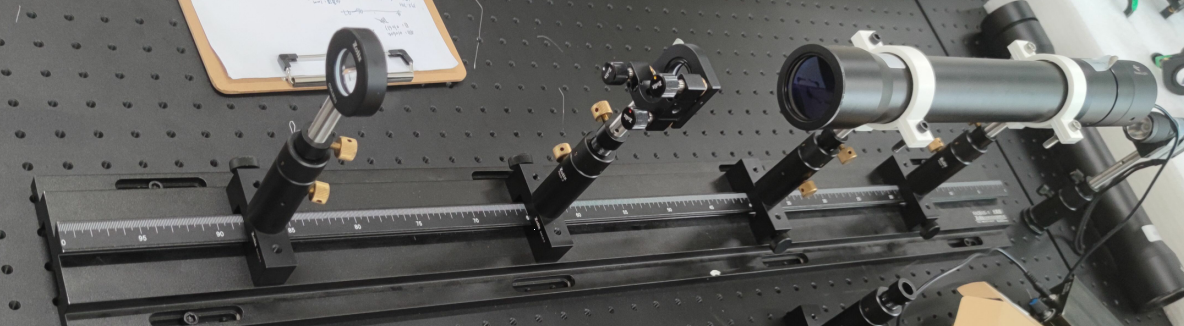
\includegraphics[width=16cm]{img/25.png}

  % 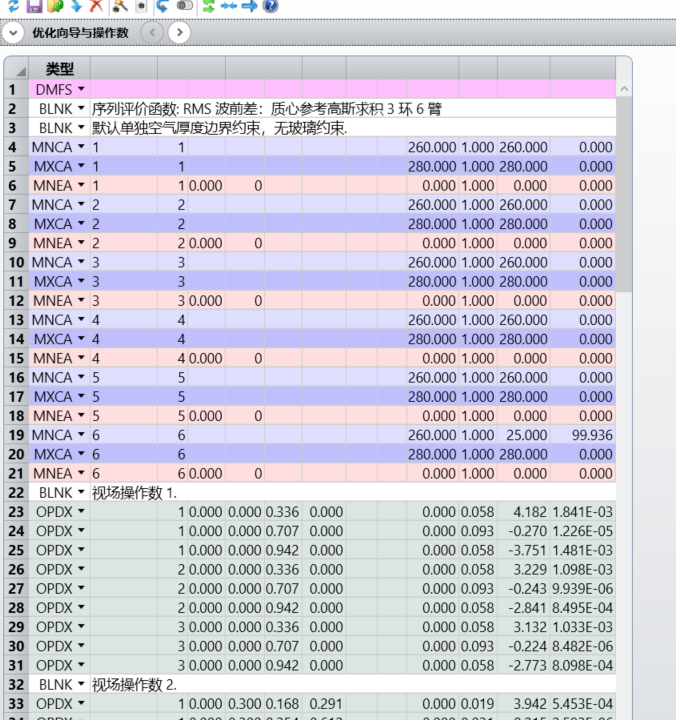
\includegraphics[width=5cm]{img/18.png}
  \caption{成像照片以及照相手机相机有光信息}
\end{figure}
经过计算可得最后有效放大倍率约为$2.51$
\section{小组名单和分工}
% \subsection{小组名单}
% 
\begin{table}[H]
  \centering
  \begin{tabular}{ccc}
  \hline
  姓名&学号&分工\\ \hline
2021251124&古翱翔& 设计仿真,实验报告撰写修改,实验\\
2021251101&姜子轩& 仿真实验优化,报告撰写,实验\\
2021251102&谭钦月& 实验数据处理,实验报告撰写,实验报告校对\\
2021251104&卢浩宇& 实验,实验报告撰写\\
2021251105&许欣茹& 实验光路搭建,实验报告撰写,实验报告校对\\ \hline
  \end{tabular}
  \caption{小组名单}
  \end{table}
% \subsection{分工}

\section{总结与预期}
在软件方面,我们小组学习了如何使用 zemax 的界面和功能,如何输入系统的参数和约束,
如何进行光线追迹和优化,如何查看系统的像差图和点扩散函数等。
% 在动手能力方面,我学习了如何根据设计的参数选择合适的透镜和支架,如何搭建光路并调整透镜的位置和角度,如何观察和拍摄像的清晰度和形状等。

我们小组学习了如何根据设计的目标和要求,
灵活地选择和组合不同类型的透镜,
如何利用软件的优化功能来改善系统的性能,如何根据实验的结果和反馈来修改和完善设计方案等。

我们小组感受到了光学是一门既简单又复杂的科学,它有着严格的数学基础和物理规律,也有着多样的现象和应用。例如,在设计望远镜时,我们不仅要考虑到透镜的形状和材料,还要考虑到光源的波长和强度,空气的折射率和湿度,透镜之间的距离和角度等多个因素。而在实验中,我们还要面对各种误差和干扰,如温度变化、灰尘污染、振动噪声等。因此,我们需要不断地学习和实践,才能掌握光学的知识和技能。

\textbf{预期效果}:
虚像的视角比物的视角增大很多,能更清晰地看到远处的物体,并感觉物体被拉近放大了。目镜物镜都使用双胶合透镜,选取玻璃GCL-010606,GCL-010631,用Zmax,调节镜片之间的距离,视场角,入瞳直径等参数,像差图中3条线相交,点列图符合要求,通过强色散玻璃与弱色散玻璃组合,使色散相互补偿,最后消除色差。

\textbf{结果}:
预期放大倍数为2.67,通过光路搭建,实验结果符合要求。
\section{附录(彩色打印实验图)}
\end{document}
